\section{函数的单调性与曲线的凹凸性}
\subsection{函数单调性的判定法}
\begin{theorem}[函数的单调性]\label{theorem:图形绘制.单调性.利用导数判定函数单调性}
%@see: 《数学分析(第二版 上册)》(陈纪修) P172 定理5.1.5(一阶导数与单调性的关系)
%@see: 《高等数学(第六版 上册)》 P146 定理1
设函数\(f\colon X\to\mathbb{R}\)在区间\(X\)上可导.
\begin{itemize}
	\item 函数\(f\)在\(X\)上单调增加的充分必要条件是:
	对于任意\(x \in X\)有\(f'(x) \geq 0\).

	\item 如果对于任意\(x \in X\)有\(f'(x) > 0\),
	则\(f\)在\(X\)上严格单调增加.

	\item 函数\(f\)在\(X\)上单调减少的充分必要条件是:
	对于任意\(x \in X\)有\(f'(x) \leq 0\).

	\item 如果对于任意\(x \in X\)有\(f'(x) < 0\),
	则\(f\)在\(X\)上严格单调减少.
\end{itemize}
%TODO proof
\end{theorem}
\begin{remark}
%@see: 《数学分析(第二版 上册)》(陈纪修) P174
%@see: 《数学分析(第二版 上册)》(陈纪修) P182 习题 11.
可以证明:若将\cref{theorem:图形绘制.单调性.利用导数判定函数单调性} 的条件
“对于任意\(x \in X\)有\(f'(x) > 0\)”
减弱为“在\(X\)中除了有限个点外,都有\(f'(x)>0\)”,
结论“\(f\)在\(X\)上严格单调增加”依然成立.
因此“对于任意\(x \in X\)有\(f'(x) > 0\)”只是“\(f\)在\(X\)上严格单调增加”的充分不必要条件.
\end{remark}

\begin{example}
%@see: 《2025年全国硕士研究生入学统一考试(数学一)》三解答题/第19题
设函数\(f(x)\)在区间\((a,b)\)内可导.
证明:导函数\(f'(x)\)在\((a,b)\)内严格单调增加的充分必要条件是
对\((a,b)\)内任意的\(x_1,x_2,x_3\),
当\(x_1<x_2<x_3\)时,
\(\frac{f(x_2)-f(x_1)}{x_2-x_1} < \frac{f(x_3)-f(x_2)}{x_3-x_2}\).
\begin{proof}
先证必要性.
% 假设\(f'(x)\)在\((a,b)\)内严格单调增加.
对\((a,b)\)内任意的\(x_1,x_2,x_3\),
当\(x_1<x_2<x_3\)时,
由\hyperref[theorem:微分中值定理.拉格朗日中值定理]{拉格朗日中值定理}可知,
存在\(\xi_1\in(x_1,x_2),\xi_2\in(x_2,x_3)\),
使得\begin{gather*}
	f'(\xi_1) = \frac{f(x_2)-f(x_1)}{x_2-x_1}, \\
	f'(\xi_2) = \frac{f(x_3)-f(x_2)}{x_3-x_2}.
\end{gather*}
因为\(f'\)严格单调增加,且\(\xi_1 < \xi_2\),
所以\(f'(\xi_1) < f'(\xi_2)\),
即\begin{equation*}
	\frac{f(x_2)-f(x_1)}{x_2-x_1}
	< \frac{f(x_3)-f(x_2)}{x_3-x_2}.
\end{equation*}

再证充分性.
% 假设对\((a,b)\)内任意的\(x_1,x_2,x_3\),
% 当\(x_1<x_2<x_3\)时,
% \(\frac{f(x_2)-f(x_1)}{x_2-x_1} < \frac{f(x_3)-f(x_2)}{x_3-x_2}\).
任取实数\(\alpha,\beta\)使之满足\(a < \alpha < \beta < b\),
必定存在\(x_0,s,t\)满足\(\alpha < s < x_0 < t < \beta\),
并且有\begin{gather*}
	\frac{f(s)-f(\alpha)}{s-\alpha} < \frac{f(x_0)-f(s)}{x_0-s},
	\tag1 \\
	\frac{f(t)-f(x_0)}{t-x_0} < \frac{f(\beta)-f(t)}{\beta-t},
	\tag2 \\
	\frac{f(x_0)-f(\alpha)}{x_0-\alpha} < \frac{f(\beta)-f(x_0)}{\beta-x_0}.
	\tag3
\end{gather*}
在(1)式中,令\(s\to\alpha^+\),得\begin{equation*}
	f'(\alpha)
	= \lim_{s\to\alpha^+} \frac{f(s)-f(\alpha)}{s-\alpha}
	\leq \lim_{s\to\alpha^+} \frac{f(x_0)-f(s)}{x_0-s}
	= \frac{f(x_0)-f(\alpha)}{x_0-\alpha}.
	\eqno(4)
\end{equation*}
在(2)式中,令\(t\to\beta^-\),得\begin{equation*}
	\frac{f(\beta)-f(x_0)}{\beta-x_0}
	= \lim_{t\to\beta^-} \frac{f(t)-f(x_0)}{t-x_0}
	\leq \lim_{t\to\beta^-} \frac{f(\beta)-f(t)}{\beta-t}
	= f'(\beta).
	\eqno(5)
\end{equation*}
由(3)(4)(5)式
可得\(f'(\alpha)<f'(\beta)\).
由\(\alpha,\beta\)的任意性可得\(f'\)在\((a,b)\)内严格单调增加.
\end{proof}
\end{example}

\begin{example}\label{example:图形绘制.单调性.函数在定义域上不单调}
%@see: 《高等数学(第六版 上册)》 P146 例2
讨论函数\(f(x) = e^x - x - 1\)的单调性.
\begin{solution}
函数\(f\)的定义域为\(\dom f = (-\infty,+\infty)\).
因为在\((-\infty,0)\)内\(f'(x)<0\),
所以\(f\)在\((-\infty,0)\)上单调减少.
因为在\((0,+\infty)\)内\(f'(x)>0\),
所以\(f\)在\((0,+\infty)\)上单调增加.
\end{solution}
\end{example}
\begin{example}\label{example:图形绘制.单调性.函数在个别点不可导}
%@see: 《高等数学(第六版 上册)》 P147 例3
讨论函数\(f(x) = \sqrt[3]{x^2}\)的单调性.
\begin{solution}
函数\(f\)的定义域为\(\dom f = (-\infty,+\infty)\).
当\(x\neq0\)时,它的导数为\begin{equation*}
	f'(x) = \frac23 x^{-\frac13}.
\end{equation*}
当\(x=0\)时,它的导数不存在.
在\((-\infty,0)\)内,\(f'(x)<0\),
因此\(f\)在\((-\infty,0)\)上单调减少.
在\((0,+\infty)\)内,\(f'(x)>0\),
因此\(f\)在\((0,+\infty)\)上单调增加.
\end{solution}
\end{example}
\begin{remark}
%@see: 《高等数学(第六版 上册)》 P147
从\cref{example:图形绘制.单调性.函数在定义域上不单调} 看出,
有些函数在它的定义区间上不是单调的.
从\cref{example:图形绘制.单调性.函数在个别点不可导} 看出,
有些函数在有限个点不可导.
因此,我们可以得出如下结论:
如果函数在定义区间上连续,
除去有限个导数不存在的点外导数存在且连续,
那么只要用方程\(f'(x) = 0\)的根
及\(f'(x)\)不存在的点
来划分函数\(f\)的定义区间,
就能保证\(f'\)在各个部分区间内保持固定符号,
因而函数\(f\)在每个部分区间上单调.
\end{remark}
\begin{example}\label{example:图形绘制.单调性.函数在个别点导数为零}
%@see: 《高等数学(第六版 上册)》 P148 例5
讨论函数\(f(x) = x^3\)的单调性.
\begin{solution}
函数\(f\)的定义域为\(\dom f = (-\infty,+\infty)\).
它的导数为\(f'(x) = 3x^2\).
显然,除了点\(x=0\)使得\(y'(x) = 0\)以外,在其余各点均有\(f'(x)>0\).
因此,函数\(f\)在\((-\infty,0]\)及\([0,\infty)\)上都是单调增加的,
从而它在整个定义域\((-\infty,+\infty)\)内是单调增加的.
\end{solution}
\end{example}
\begin{remark}
%@see: 《高等数学(第六版 上册)》 P148
从\cref{example:图形绘制.单调性.函数在个别点导数为零} 可以看出:
如果\(f'\)在某区间内的有限个点处为零,
在其余各点处均为正(或负)时,
那么\(f\)在该区间上仍旧是单调增加(或单调减少)的.
\end{remark}

\begin{example}
%@see: 《高等数学(第六版 上册)》 P148 例6
证明:当\(x > 1\)时,\(2 \sqrt{x} > 3 - \frac{1}{x}\).
\begin{proof}
令\(f(x) = 2 \sqrt{x} - \left(3 - \frac{1}{x}\right)\),
则\begin{equation*}
	f'(x) = \frac{1}{\sqrt{x}} - \frac{1}{x^2}
	= \frac{1}{x^2} (x \sqrt{x} - 1).
\end{equation*}

\(f\)在\([1,+\infty)\)上连续,在\((1,+\infty)\)内\(f'(x) > 0\),
因此在\([1,+\infty)\)上\(f\)单调增加,
从而当\(x > 1\)时,\(f(x) > f(1) = 0\),
即\(2 \sqrt{x} - \left(3 - \frac{1}{x}\right) > 0\),
\(2 \sqrt{x} > 3 - \frac{1}{x}\).
\end{proof}
\end{example}

\begin{example}
%@see: 《数学分析(第二版 上册)》(陈纪修) P182 习题 12. (1)
证明\DefineConcept{若尔当不等式}:
当\(0<x<\frac\pi2\)时,
有\begin{equation}\label{equation:微分中值定理.若尔当不等式}
	\frac2\pi < \frac{\sin x}{x} < 1.
\end{equation}
\begin{proof}
设\(f(x) = \frac{\sin x}{x}\ (0<x<\frac\pi2)\),
那么\(f'(x) = \frac{x \cos x - \sin x}{x^2}\).
又设\(g(x) = x \cos x - \sin x\),
那么\begin{equation*}
	g'(x) = \cos x - x \sin x - \cos x = -x \sin x < 0\ (0<x<\frac\pi2),
\end{equation*}
说明\(g\)是\((0,\frac\pi2)\)上的单调减少函数.
又因为\(g(0) = 0\),
从而\(g(x) < 0\ (0<x<\frac\pi2)\),
所以\(f'(x) < 0\),
\(f\)也是\((0,\frac\pi2)\)上的单调减少函数.
应用洛必达法则,得\begin{equation*}
	\lim_{x\to0^+} f(x)
	= \lim_{x\to0^+} \cos x
	= 1.
\end{equation*}
再因为\begin{equation*}
	\lim_{x\to\frac\pi2^-} f(x)
	= \frac{\sin(\pi/2)}{\pi/2}
	= \frac2\pi,
\end{equation*}
所以\begin{equation*}
	\frac2\pi < \frac{\sin x}{x} < 1.
	\qedhere
\end{equation*}
\end{proof}
\end{example}

\begin{example}
证明:
当\(0<x<\frac\pi2\)时,
有\begin{equation}\label{equation:单调性.正切不等式}
	\tan x > x.
\end{equation}
\begin{proof}
设\(f(x) = \tan x - x\ (0<x<\frac\pi2)\).
求导得\(f'(x) = \sec^2 x - 1 = \tan^2 x\).
显然\(f'(x) > 0\ (0<x<\frac\pi2)\),
\(f\)是\((0,\frac\pi2)\)上的严格单调增加函数.
又因为\(f(0) = \tan0 - 0 = 0\),
所以\(f(x) = \tan x - x > 0\ (0<x<\frac\pi2)\),
即\(\tan x > x\ (0<x<\frac\pi2)\).
\end{proof}
\end{example}

\begin{example}
%@see: 《数学分析(第二版 上册)》(陈纪修) P182 习题 12. (5)
证明不等式\begin{equation*}
	\frac1{2^{p-1}}
	\leq x^p + (1-x)^p
	\leq 1
	\quad(0 \leq x \leq 1, p>1).
\end{equation*}
%TODO proof
\end{example}
\begin{example}
%@see: 《数学分析(第二版 上册)》(陈纪修) P183 习题 12. (6)
证明不等式\begin{equation*}
	\frac{\tan x}{x} > \frac{x}{\sin x}
	\quad(0 < x < \pi/2).
\end{equation*}
%TODO proof
\end{example}

\begin{example}
%@see: https://www.bilibili.com/video/BV19YpbepEGF
设数列\(\{x_n\}\)有递推公式\(x_{n+1} = f(x_n)\ (n=1,2,\dotsc)\).
证明:\begin{itemize}
	\item 如果\(f'(x) > 0\),则\(\{x_n\}\)是单调的.
	\item 如果\(f'(x) < 0\),则\(\{x_n\}\)不是单调的.
\end{itemize}
\begin{proof}
假设\(f'(x) > 0\)且\(x_2 \geq x_1\),
那么\(x_3 = f(x_2) \geq f(x_1) = x_2\),
利用数学归纳法可证\(x_{n+1} \geq x_n\)对\(n=1,2,\dotsc\)成立.
因此,当\(f'(x) > 0\)时,\(\{x_n\}\)是单调的.

假设\(f'(x) < 0\)且\(x_2 \geq x_1\),
那么\(x_3 = f(x_2) \leq f(x_1) = x_2\),
显然,当\(f'(x) < 0\)时,\(\{x_n\}\)不是单调的.
\end{proof}
\end{example}

\begin{example}
%@see: 《数学分析(第二版 上册)》(陈纪修) P177 例5.1.5
判别\(e^\pi\)与\(\pi^e\)的大小关系.
\begin{solution}
对于正实数\(a,b\),有\begin{align*}
	a^b > b^a
	&\iff
	b \ln a = \ln a^b > \ln b^a = a \ln b \\
	&\iff
	\frac{\ln a}{a} > \frac{\ln b}{b}.
\end{align*}
下面考察函数\(f(x) = \frac{\ln x}{x}\)的单调性.
求导得\begin{equation*}
	f'(x) = \frac{1 - \ln x}{x^2}.
\end{equation*}
令\(f'(x) > 0\)得\(0 < x < e\).
由\cref{theorem:图形绘制.单调性.利用导数判定函数单调性} 可知,
函数\(f\)在\((0,e)\)上严格单调增加,在\((e,+\infty)\)上严格单调减少.
由于\(\pi > e\),所以\begin{equation*}
	\frac{\ln e}{e} > \frac{\ln \pi}{\pi},
\end{equation*}
那么\(e^\pi > \pi^e\).
\end{solution}
\end{example}

\subsection{曲线的凹凸性与拐点}
\begin{definition}\label{definition:函数图像的绘制.凹凸性的定义}
%@see: 《数学分析(第7版 第一卷)》(卓里奇) P202 定义1
%@see: 《数学分析(第7版 第一卷)》(卓里奇) P203 定义2
%@see: 《数学分析(第二版 上册)》(陈纪修) P173 定义5.1.2
设函数\(f\colon D\to\mathbb{R}\),其中\(D=(a,b)\subset\mathbb{R}\).

若\begin{equation*}
	(\forall x_1,x_2 \in D)
	(\forall \lambda \in [0,1])
	[
		f(\lambda x_1 + (1-\lambda) x_2)
		\leq
		\lambda f(x_1) + (1-\lambda) f(x_2)
	],
\end{equation*}
则称“\(f\)是\(D\)上的\DefineConcept{凹函数}(convex function)”.

若\begin{equation*}
	(\forall x_1,x_2 \in D)
	(\forall \lambda \in [0,1])
	[
		f(\lambda x_1 + (1-\lambda) x_2)
		\geq
		\lambda f(x_1) + (1-\lambda) f(x_2)
	],
\end{equation*}
则称“\(f\)是\(D\)上的\DefineConcept{凸函数}(concave function)
\footnote{有的书把凹函数称为\DefineConcept{下凸函数},
把凸函数称为\DefineConcept{上凸函数}.
% 例如:
% 《数学分析(第二版 上册)》(陈纪修)
有的书反过来把凹函数称为凸函数,
把凸函数称为凹函数.
% 例如:
% 《数学分析(第7版 第一卷)》(卓里奇)
}”.

若\begin{equation*}
	(\forall x_1,x_2 \in D)
	[
		x_1 \neq x_2
		\implies
		(\forall \lambda \in (0,1))
		[
			f(\lambda x_1 + (1-\lambda) x_2)
			<
			\lambda f(x_1) + (1-\lambda) f(x_2)
		]
	],
\end{equation*}
则称“\(f\)是\(D\)上的\DefineConcept{严格凹函数}%
(strictly convex function)”.

若\begin{equation*}
	(\forall x_1,x_2 \in D)
	[
		x_1 \neq x_2
		\implies
		(\forall \lambda \in (0,1))
		[
			f(\lambda x_1 + (1-\lambda) x_2)
			>
			\lambda f(x_1) + (1-\lambda) f(x_2)
		]
	],
\end{equation*}
则称“\(f\)是\(D\)上的\DefineConcept{严格凸函数}%
(strictly concave function)”.
%@see: https://mathworld.wolfram.com/ConvexFunction.html
%@see: https://mathworld.wolfram.com/ConcaveFunction.html
%@see: https://doi.org/10.1007/978-3-030-41804-5
\end{definition}

\begin{figure}[hbt]
	\centering
	\def\subwidth{.45\linewidth}
	\begin{subfigure}[b]{\subwidth}
		\centering
		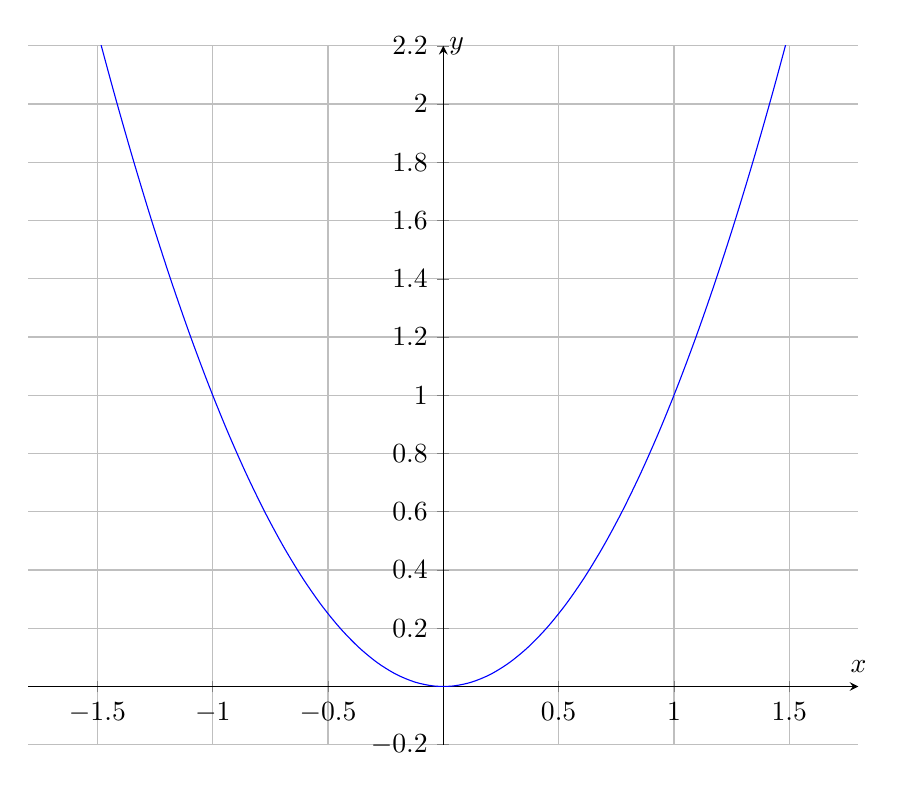
\begin{tikzpicture}
			\begin{axis}[
				xmin=-1.5,xmax=1.5,
				ymin=0,ymax=2,
				width=\textwidth,
				grid=both,
				axis lines=middle,
				xlabel=$x$,
				ylabel=$y$,
				enlarge x limits=0.1,
				enlarge y limits=0.1,
				x label style={at={(ticklabel* cs:1.00)}, inner sep=5pt, anchor=south},
				y label style={at={(ticklabel* cs:1.00)}, inner sep=2pt, anchor=west},
			]
				\addplot[color=blue,samples=50,smooth,domain=-2:2]{x^2};
			\end{axis}
		\end{tikzpicture}
		\caption{函数$f(x) = x^2$是严格凹函数}
	\end{subfigure}~\begin{subfigure}[b]{\subwidth}
		\centering
		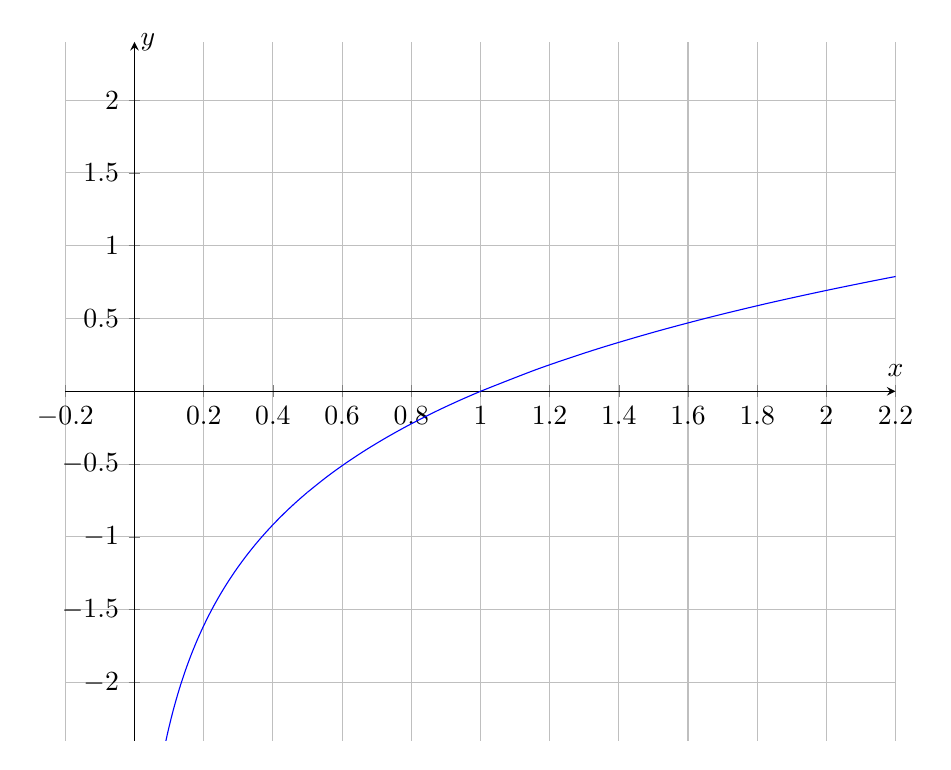
\begin{tikzpicture}
			\begin{axis}[
				xmin=0,xmax=2,
				ymin=-2,ymax=2,
				width=\textwidth,
				grid=both,
				axis lines=middle,
				xlabel=$x$,
				ylabel=$y$,
				enlarge x limits=0.1,
				enlarge y limits=0.1,
				x label style={at={(ticklabel* cs:1.00)}, inner sep=5pt, anchor=south},
				y label style={at={(ticklabel* cs:1.00)}, inner sep=2pt, anchor=west},
			]
				\addplot[color=blue,samples=30,smooth,domain=.01:.5]{ln(x)};
				\addplot[color=blue,samples=10,smooth,domain=.5:1]{ln(x)};
				\addplot[color=blue,samples=10,smooth,domain=1:2.5]{ln(x)};
			\end{axis}
		\end{tikzpicture}
		\caption{函数$f(x) = \ln x$是严格凸函数}
	\end{subfigure}
	\caption{}
\end{figure}

\begin{definition}
设函数\(f\colon D\to\mathbb{R}\).

若\begin{equation*}
	(\exists\alpha>0)
	[\text{函数\(g(x)=f(x)-\alpha\abs{x}^2\)是凹函数}],
\end{equation*}
则称“\(f(x)\)是\(D\)上的\DefineConcept{强凹函数}
(strongly convex function)”.

若\begin{equation*}
	(\exists\alpha>0)
	[\text{函数\(g(x)=f(x)-\alpha\abs{x}^2\)是凸函数}],
\end{equation*}
则称“\(f(x)\)是\(D\)上的\DefineConcept{强凸函数}
(strongly concave function)”.
%@see: https://www.princeton.edu/~aaa/Public/Teaching/ORF523/S16/ORF523_S16_Lec7_gh.pdf
\end{definition}

\begin{proposition}
强凹(凸)函数必定严格凹(凸).
\end{proposition}

\begin{proposition}[延森不等式]
%@see: 《数学分析(第7版 第一卷)》(卓里奇) P207 命题7(延森不等式)
%@see: 《数学分析(第二版 上册)》(陈纪修) P176 定理5.1.8
%@see: 《数学分析(第二版 上册)》(陈纪修) P184 习题 24.(Jensen不等式)
设函数\(f\colon(a,b)\to\mathbb{R}\),
\(\AutoTuple{x}{n}\in(a,b)\),
\(\AutoTuple{k}{n}\in(0,1)\)
且\(\AutoTuple{k}{n}[+]=1\).
\begin{itemize}
	\item 如果\(f\)是凸函数,
	则\begin{equation*}
		%@see: 《数学分析(第7版 第一卷)》(卓里奇) P207 (15)
		f(k_1 x_1 + \dotsb + k_n x_n)
		\geq
		k_1 f(x_1) + \dotsb + k_n f(x_n).
	\end{equation*}
	\item 如果\(f\)是凹函数,
	则\begin{equation*}
		%@see: 《数学分析(第7版 第一卷)》(卓里奇) P207 (14)
		f(k_1 x_1 + \dotsb + k_n x_n)
		\leq
		k_1 f(x_1) + \dotsb + k_n f(x_n).
	\end{equation*}
\end{itemize}
如果\(\AutoTuple{k}{n}\)均不为零,
那么上述两条不等式的取等条件就是\(x_1=x_2=\dotsb=x_n\).
\begin{proof}
这里只证“\(f\)是凹函数”的情形.

假设\(f\)是凹函数.
当\(n=2\)时,条件、结论与\cref{definition:函数图像的绘制.凹凸性的定义} 相同,自然成立.

利用数学归纳法.
假设当\(n=m-1\ (m\geq3)\)时结论成立.
当\(n=m\)时,
记\(p = k_2 + \dotsb + k_n\),
则\begin{equation*}
	\frac{k_2}{p} + \dotsb + \frac{k_n}{p} = 1,
\end{equation*}
于是\begin{align*}
	f(k_1 x_1 + \dotsb + k_n x_n)
	&= f\left( k_1 x_1 + p \left( \frac{k_2}{p} x_2 + \dotsb + \frac{k_n}{p} x_n \right) \right) \\
	&\leq k_1 f(x_1) + p f\left( \frac{k_2}{p} x_2 + \dotsb + \frac{k_n}{p} x_n \right),
\end{align*}
这里\(k_1 + p = 1\)
且\(\frac{k_2}{p} x_2 + \dotsb + \frac{k_n}{p} x_n \in (a,b)\).
再由归纳假设可知\begin{equation*}
	f\left( \frac{k_2}{p} x_2 + \dotsb + \frac{k_n}{p} x_n \right)
	\leq \frac{k_2}{p} f(x_2) + \dotsb + \frac{k_n}{p} f(x_n),
\end{equation*}
所以\begin{align*}
	f(k_1 x_1 + \dotsb + k_n x_n)
	&\leq k_1 f(x_1) + p f\left( \frac{k_2}{p} x_2 + \dotsb + \frac{k_n}{p} x_n \right) \\
	&\leq k_1 f(x_1) + k_2 f(x_2) + \dotsb + k_n f(x_n).
	\qedhere
\end{align*}
\end{proof}
\end{proposition}

\begin{theorem}[曲线凹凸的判定]\label{theorem:微分中值定理.曲线凹凸的判定}
%@see: 《数学分析(第二版 上册)》(陈纪修) P173 定理5.1.6(二阶导数与凹凸性的关系)
设\(f\colon X\to\mathbb{R}\)在区间\(X\)内具有二阶导数.
\begin{itemize}
	\item 若在\(X\)内\(f''(x)>0\),
	则\(f\)是\(X\)上的严格凹函数.
	\item 若在\(X\)内\(f''(x)<0\),
	则\(f\)是\(X\)上的严格凸函数.
\end{itemize}
\begin{proof}
在情形1,设\(x_1\)和\(x_2\)为\(X\)内任意两点,且\(x_1 < x_2\),
记\(\frac{x_1 + x_2}{2} = x_0\),
并记\(x_2 - x_0 = x_0 - x_1 = h\),
则\(x_1 = x_0 - h\),\(x_2 = x_0 + h\),
由拉格朗日中值公式,
得\begin{gather*}
	f(x_0 + h) - f(x_0) = f'(x_0 + \theta_1 h) h, \\
	f(x_0) - f(x_0 - h) = f'(x_0 - \theta_2 h) h,
\end{gather*}
其中\(0 < \theta_1 < 1\),\(0 < \theta_2 < 1\).
两式相减,即得\begin{equation*}
	f(x_0 + h) + f(x_0 - h) - 2 f(x_0)
	= [ f'(x_0 + \theta_1 h) - f'(x_0 - \theta_2 h) ] h.
\end{equation*}
对\(f'(x)\)在区间\([x_0 - \theta_2 h,x_0 + \theta_1 h]\)上再利用拉格朗日中值公式,
得\begin{equation*}
	[ f'(x_0 + \theta_1 h) - f'(x_0 - \theta_2 h) ] h
	= f''(\xi) (\theta_1 + \theta_2) h^2,
\end{equation*}
其中\(x_0 - \theta_2 h < \xi < x_0 + \theta_1 h\).
按情形1的假设,\(f''(\xi) > 0\),
故有\begin{equation*}
	f(x_0 + h) + f(x_0 - h) - 2 f(x_0) > 0,
\end{equation*}
即\begin{equation*}
	\frac{f(x_0 + h) + f(x_0 - h)}{2} > f(x_0),
\end{equation*}
亦即\begin{equation*}
	\frac{f(x_1) + f(x_2)}{2} > f\left(\frac{x_1 + x_2}{2}\right),
\end{equation*}
所以\(f(x)\)在\(X\)上的图形是凹的.

类似地可证情形2.
\end{proof}
\end{theorem}
\begin{remark}
%@see: 《数学分析(第二版 上册)》(陈纪修) P174
可以证明:若将\cref{theorem:微分中值定理.曲线凹凸的判定} 的条件
“在\(X\)内\(f''(x)>0\)”
减弱为“在区间\(X\)中除了有限个点外,都有\(f''(x)>0\)”,
结论“\(f\)是\(X\)上的严格凹函数”依然成立.
因此“在\(X\)内\(f''(x)>0\)”只是“\(f\)是\(X\)上的严格凹函数”的充分不必要条件.
\end{remark}

\begin{definition}\label{definition:单调性和凹凸性.拐点}
%@see: 《数学分析(第二版 上册)》(陈纪修) P175
如果函数\(f\)的凹凸性在点\(x_0\)左邻域、右邻域相反,
那么就称“点\(x_0\)是函数\(f\)的\DefineConcept{拐点}(inflection point)”
%@see: https://mathworld.wolfram.com/InflectionPoint.html
“点\((x_0,f(x_0))\)是曲线\(y=f(x)\)的拐点”.
\end{definition}

\begin{example}
函数\(f(x) = x^3\)以\(x=0\)为拐点.
函数\(g(x) = \abs{x(x-1)}\)以\(x=0\)和\(x=1\)为拐点.
\end{example}

\begin{theorem}\label{theorem:单调性和凹凸性.拐点的判定}
%@see: 《数学分析(第二版 上册)》(陈纪修) P175 定理5.1.7
设\(f\colon X\to\mathbb{R}\)在区间\(X\)上连续,
存在\(\delta>0\)使得\((x_0-\delta,x_0+\delta) \subseteq X\).
\begin{itemize}
	\item 设\(f\)在\((x_0-\delta,x_0)\cup(x_0,x_0+\delta)\)上二阶可导.
	\begin{itemize}
		\item 若\(f''\)在\((x_0-\delta,x_0)\)与\((x_0,x_0+\delta)\)上的符号相反,
		则点\(x_0\)是函数\(f\)的拐点.
		\item 若\(f''\)在\((x_0-\delta,x_0)\)与\((x_0,x_0+\delta)\)上的符号相同,
		则点\(x_0\)不是函数\(f\)的拐点.
	\end{itemize}

	\item 设\(f\)在\((x_0-\delta,x_0+\delta)\)上二阶可导.
	若点\(x_0\)是函数\(f\)的拐点,
	则\(f''(x_0) = 0\).
\end{itemize}
\begin{proof}
假设\(f\)在\((x_0-\delta,x_0+\delta)\)上二阶可导,
且点\(x_0\)是函数\(f\)的拐点.
不妨设\(f\)是\((x_0-\delta,x_0)\)上的凹函数,\((x_0,x_0+\delta)\)上的凸函数.
由\cref{theorem:微分中值定理.曲线凹凸的判定} 可知
在\((x_0-\delta,x_0)\)上\(f''(x)\geq0\),
在\((x_0,x_0+\delta)\)上\(f''(x)\leq0\);
换言之,\(f'\)在\((x_0-\delta,x_0)\)上单调增加,在\((x_0,x_0+\delta)\)上单调减少;
因此点\(x_0\)是\(f'\)的极大值点.
因为\(f''\)在点\(x_0\)有定义,
那么由\hyperref[theorem:微分中值定理.费马引理]{费马引理}可知\(f''(x_0)=0\).
\end{proof}
\end{theorem}
\begin{remark}
“\(f''(x_0) = 0\)”是二阶可导函数曲线拐点的必要不充分条件.
例如,曲线\(y = x^4\)上的点\((0,0)\)就满足条件\(f''(0) = 0\),但它不是拐点.
又例如,曲线\(y = x^{1/3}\)在点\(x=0\)不可导,但是点\((0,0)\)是它的拐点.
\end{remark}

由\cref{theorem:微分中值定理.曲线凹凸的判定} 可知,由\(f''(x)\)的符号可以判定曲线的凹凸性.
因此,如果\(f''(x)\)在\(x_0\)的左右两侧邻近异号,那么点\((x_0,f(x_0))\)就是曲线的一个拐点,
所以,要寻找拐点,只要找出\(f''(x)\)符号发生变化的分界点即可.
如果\(f(x)\)在区间\((a,b)\)内具有二阶连续导数,那么在这样的分界点处必然有\(f''(x)=0\);
除此以外,\(f(x)\)的二阶导数不存在的点,也有可能是\(f''(x)\)的符号发生变化的分界点.

综合以上分析,我们可以按下列步骤来判定区间\(I\)上的连续曲线\(y=f(x)\)的拐点:
\begin{algorithm}[判定连续曲线的拐点]
\hfill
\begin{enumerate}
	\item 求\(f''(x)\);

	\item 令\(f''(x) = 0\),解出这个方程在区间\(I\)内的实根,
	并求出在区间\(I\)内\(f''(x)\)不存在的点;

	\item 对于上一步中求出的每一个实根或二阶导数不存在的点\(x_0\),
	检查\(f''(x)\)在\(x_0\)左右两侧邻近的符号,
	那么当两侧的符号相反时,点\((x_0,f(x_0))\)就是拐点;
	当两侧的符号相同时,点\((x_0,f(x_0))\)不是拐点.
\end{enumerate}
\end{algorithm}

\begin{example}
证明:当\(x>0\),\(y>0\),\(x \neq y\),且\(n>1\)时,
成立\begin{equation}\label{equation:微分中值定理.平均数的比较1}
	\frac{1}{2} (x^n+y^n) > \left(\frac{x+y}{2}\right)^n.
\end{equation}
\begin{proof}
设\(f(x) = x^n\),那么\(f'(x) = n x^{n-1}\),\(f''(x) = n(n-1) x^{n-2}\).
由指数函数的性质可知,
当\(x > 0\)时,\(\forall \mu \in \mathbb{R}\)都有\(x^{\mu} > 0\)成立,
故当\(n > 1\)时,\(n(n-1)>0\),\(f''(x) = n(n-1) x^{n-1} > 0\)成立,
即\(f(x)\)在\((0,+\infty)\)上是凹函数,
那么\(\forall x,y>0\),
只要\(x \neq y\),
就有\begin{equation*}
	\frac{f(x)+f(y)}{2} = \frac{x^n+y^n}{2}
	> \left(\frac{x+y}{2}\right)^n = f\left(\frac{x+y}{2}\right)
\end{equation*}成立.
\end{proof}
\end{example}

\begin{example}
证明:当\(x \neq y\)时,有\begin{equation}
	\frac{e^x + e^y}{2} > e^{\frac{x+y}{2}}.
\end{equation}
\begin{proof}
设\(f(x) = e^x\),那么\(f'(x) = f''(x) = e^x > 0\ (x\in\mathbb{R})\),可知\(f(x)\)是凹函数.
因此\begin{equation*}
	f\left(\frac{x+y}{2}\right) = e^{\frac{x+y}{2}}
	< \frac{e^x+e^y}{2} = \frac{f(x)+f(y)}{2}.
	\qedhere
\end{equation*}
\end{proof}
\end{example}

\begin{example}[杨格不等式]\label{example:函数图像的绘制.杨格不等式}
%@see: 《数学分析(第二版 上册)》(陈纪修) P179 例5.1.8
设\(a,b\geq0\),正数\(p,q\)满足\(\frac1p+\frac1q=1\).
证明:\begin{equation*}
	a b \leq \frac1p a^p + \frac1q b^q.
\end{equation*}
当且仅当\(a^p = b^q\)时上式取“\(=\)”号.
\begin{proof}
当\(a=0\)或\(b=0\)时,上式显然成立.

下面考虑\(a,b>0\)的情形.
由于函数\(f(x) = \ln x\ (x>0)\)的一阶导数\begin{equation*}
	f'(x) = \frac1x > 0,
\end{equation*}
二阶导数\begin{equation*}
	f''(x) = -\frac1{x^2} < 0,
\end{equation*}
所以\(f\)是\((0,+\infty)\)上的严格单调增加的严格凸函数.
那么由\cref{definition:函数图像的绘制.凹凸性的定义} 得\begin{equation*}
	\ln(ab) = \frac1p \ln a^p + \frac1q \ln b^q
	\leq \ln\left( \frac1p a^p + \frac1q b^q \right),
\end{equation*}
因此\begin{equation*}
	ab \leq \frac1p a^p + \frac1q b^q.
	\qedhere
\end{equation*}
\end{proof}
\end{example}
\begin{remark}
\cref{example:函数图像的绘制.杨格不等式}
利用微分学重新证明了\hyperref[theorem:不等式.杨格不等式]{杨格不等式}.
\end{remark}
\begin{remark}
类似地可以证明对于任意正数\(x_1,\dotsc,x_n\),成立\begin{equation*}
	\frac{\ln x_1 + \dotsb + \ln x_n}{n}
	\leq \ln\left( \frac{x_1 + \dotsb + x_n}{n} \right),
\end{equation*}
从而有\begin{equation*}
	\sqrt[n]{x_1 \dotsm x_n}
	\leq \frac{x_1 + \dotsb + x_n}{n}.
\end{equation*}
\end{remark}

\begin{example}[赫尔德不等式]\label{example:不等式.赫尔德不等式}
%@see: 《数学分析教程 (第3版 上册)》(史济怀) P306 例8
设\(\AutoTuple{x}{n},\AutoTuple{y}{n}\geq0\),\(p,q>1\),
且满足\(\frac{1}{p}+\frac{1}{q}=1\),
则
\def\s{\sum_{i=1}^n}%
\def\sp#1#2#3{\left( \s #1^#2 \right)^{#3/#2}}%
\begin{equation}
	\s x_i y_i
	\leq
	\sp{x_i}{p}{1} \sp{y_i}{q}{1},
\end{equation}
当且仅当存在常数\(\lambda\)使得\(a_i^p = \lambda b_i^q\ (i=1,2,\dotsc,n)\)时取“\(=\)”号.
\begin{proof}
令\begin{equation*}
	a_j = x_j \sp{x_i}{p}{-1}, \qquad
	b_j = y_j \sp{y_i}{q}{-1}.
\end{equation*}
那么根据\cref{example:函数图像的绘制.杨格不等式} 得到\begin{equation*}
	\s a_i b_i \leq \s \left( \frac{a_i^p}{p} + \frac{b_i}{q} \right)
	\leq \frac{1}{p} + \frac{1}{q} = 1.
	\qedhere
\end{equation*}
\end{proof}
\end{example}

\begin{example}[闵可夫斯基不等式]\label{example:不等式.闵可夫斯基不等式}
设\(\AutoTuple{x}{n},\AutoTuple{y}{n}\in\mathbb{R}\),\(p\geq1\),则
\def\s{\sum_{i=1}^n}%
\def\sumonly#1{\s \abs{#1}^p}%
\newcommand\sumpower[2][1]{\left( \sumonly{#2} \right)^{\frac{#1}{p}}}%
\begin{equation}
	\sumpower{x_i+y_i} \leq \sumpower{x_i} + \sumpower{y_i}.
\end{equation}
\begin{proof}
利用\cref{example:不等式.赫尔德不等式} 就有\begin{align*}
	&\hspace{-20pt}\sumonly{x_i+y_i}
	= \s \abs{x_i+y_i} \abs{x_i+y_i}^{p-1}
	\leq \s (\abs{x_i}+\abs{y_i}) \abs{x_i+y_i}^{p-1} \\
	&\leq \sumpower{x_i} \sumpower[p-1]{x_i+y_i}
	+ \sumpower{y_i} \sumpower[p-1]{x_i+y_i}.
\end{align*}
整理即得欲证不等式.
\end{proof}
\end{example}
